%
%
%
%
%
%
%
%
%
%
%
%
%
\ZSFChapterDensity{0.60}
\ZSFBoxesBreakableOn
\StartChapter{Anhang}
\allowdisplaybreaks[4]

\SubsectionBar{Stammfunktionen \& Grundintegrale\ZSFScriptRef{72}}
\ZSFindex{Stammfunktionen}
\begin{formulabox}[Grund- und rationale Integrale][align=left]
    $\displaystyle \int x^n\,dx = \frac{1}{n+1}x^{n+1}+C$\par
    \ZSFsep
    $\displaystyle \int \frac{1}{x^n}\,dx = -\frac{1}{n-1}\cdot\frac{1}{x^{n-1}}+C$\par
    \ZSFsep
    \ZSFformulaline{\int g'(\ZSFqParameterA{a}x+\ZSFqParameterB{b})\,dx = \frac{1}{\ZSFqParameterA{a}}\,g(\ZSFqParameterA{a}x+\ZSFqParameterB{b})+C}{$\ZSFmhlC{u=\ZSFqParameterA{a}x+\ZSFqParameterB{b}}$}
    \ZSFsep
    \ZSFformulaline{\int \frac{f'(x)}{f(x)}\,dx = \ln(|f(x)|)+C}{$\ZSFmhlC{u=f(x)}$}
    \ZSFsep
    \ZSFformulaline{\int \frac{1}{\ZSFqParameterA{a}x+\ZSFqParameterB{b}}\,dx = \frac{1}{\ZSFqParameterA{a}}\ln(|\ZSFqParameterA{a}x+\ZSFqParameterB{b}|)+C}{$\ZSFmhlC{u=\ZSFqParameterA{a}x+\ZSFqParameterB{b}}$}
    \ZSFsep
    \ZSFformulaline{\int \frac{x}{x+\ZSFqParameterB{b}}\,dx = x-\ZSFqParameterB{b}\ln(|x+\ZSFqParameterB{b}|)+C}{$\ZSFmhlC{u=x+\ZSFqParameterB{b}}$}
    \ZSFsep
    \ZSFformulaline{\int \frac{1}{(x-\ZSFqParameterA{a})(x-\ZSFqParameterB{b})}\,dx = \frac{1}{\ZSFqParameterA{a}-\ZSFqParameterB{b}}\ln\!\left(\left|\frac{x-\ZSFqParameterA{a}}{x-\ZSFqParameterB{b}}\right|\right)+C}{\text{PBZ}}
    \ZSFsep
    \ZSFformulaline{\int \frac{1}{\ZSFqParameterA{a}^2+x^2}\,dx = \frac{1}{\ZSFqParameterA{a}}\arctan\!\left(\frac{x}{\ZSFqParameterA{a}}\right)+C}{$\ZSFmhlA{x=\ZSFqParameterA{a}\tan u}$}
    \ZSFsep
    \ZSFformulaline{\int \frac{1}{\ZSFqParameterA{a}^2-x^2}\,dx = \frac{1}{2\ZSFqParameterA{a}}\ln\!\left(\left|\frac{\ZSFqParameterA{a}+x}{\ZSFqParameterA{a}-x}\right|\right)+C}{\text{PBZ}}
    \ZSFsep
    \ZSFformulaline{\int \frac{x}{\ZSFqParameterA{a}x^2+\ZSFqParameterB{b}}\,dx = \frac{1}{2\ZSFqParameterA{a}}\ln(|\ZSFqParameterA{a}x^2+\ZSFqParameterB{b}|)+C}{$\ZSFmhlC{u=\ZSFqParameterA{a}x^2+\ZSFqParameterB{b}}$}
    \ZSFsep
    \ZSFformulaline{\int \frac{1}{1+x^2}\,dx = \arctan(x)+C}{$\ZSFmhlA{x=\tan u}$}
    \ZSFsep
    \ZSFformulaline{\int \frac{x}{x^4+3}\,dx = \frac{\sqrt{3}}{6}\arctan\!\left(\frac{x^2}{\sqrt{3}}\right)+C}{$\ZSFmhlC{u=x^2}$}
    \ZSFsep
    \ZSFformulaline{\int \frac{1}{x^3+x}\,dx = \ln(|x|)-\frac{1}{2}\ln(x^2+1)+C}{\text{PBZ}}
    \ZSFsep
    \ZSFformulaline{\int \frac{1}{x^2+x}\,dx = \ln(|x|)-\ln(|x+1|)+C}{\text{PBZ}}
    \ZSFsep
    \ZSFformulaline{\int \frac{1}{1-x^2}\,dx = \Artanh(x)+C}{$\ZSFmhlA{x=\tanh u}$}
\end{formulabox}

\begin{formulabox}[Wurzelfunktionen][align=left]
    \ZSFformulaline{\int \sqrt{x\pm \ZSFqParameterA{a}}\,dx = \frac{2}{3}(x\pm \ZSFqParameterA{a})^{3/2}+C}{$\ZSFmhlC{u=x\pm\ZSFqParameterA{a}}$}
    \ZSFsep
    \ZSFformulaline{\int \sqrt{1-x^2}\,dx = \frac{1}{2}\bigl(\arcsin(x)+x\sqrt{1-x^2}\bigr)+C}{$\ZSFmhlA{x=\sin u}$}
    \ZSFsep
    $\displaystyle \int \sqrt{\ZSFqParameterA{a}^2-x^2}\,dx = \frac{1}{2}\ZSFqParameterA{a}^2\arcsin\!\left(\frac{x}{\ZSFqParameterA{a}}\right) + \frac{1}{2}x\sqrt{\ZSFqParameterA{a}^2-x^2}+C$\par
    \ZSFsep
    \ZSFformulaline{\int 2x\sqrt{\ZSFqParameterA{a}+x^2}\,dx = \frac{2}{3}(\ZSFqParameterA{a}+x^2)^{3/2}+C}{$\ZSFmhlC{u=\ZSFqParameterA{a}+x^2}$}
    \ZSFsep
    $\displaystyle \int \sqrt{x^2+1}\,dx = \frac{1}{2}\bigl(\Arsinh(x)+x\sqrt{1+x^2}\bigr)+C$\par
    \ZSFsep
    \ZSFformulaline{\int \frac{1}{\sqrt{1-x^2}}\,dx = \arcsin(x)+C}{$\ZSFmhlA{x=\sin u}$}
    \ZSFsep
    \ZSFformulaline{\int \frac{1}{\sqrt{x^2-1}}\,dx = \mathrm{arcosh}(x)+C}{$\ZSFmhlB{x=\cosh u}$}
    \ZSFsep
    \ZSFformulaline{\int \frac{x}{\sqrt{x^2-1}}\,dx = \sqrt{x^2-1}+C}{$\ZSFmhlC{u=x^2-1}$}
    \ZSFsep
    \ZSFformulaline{\int \frac{1}{\sqrt{x^2+1}}\,dx = \Arsinh(x)+C}{$\ZSFmhlB{x=\sinh u}$}
    \ZSFsep
    \ZSFformulaline{\int \frac{x}{\sqrt{1-x^2}}\,dx = -\sqrt{1-x^2}+C}{$\ZSFmhlC{u=1-x^2}$}
    \ZSFsep
    \ZSFformulaline{\int \frac{1}{\sqrt{x^2-4}}\,dx = \ln\!\left(\left|x+\sqrt{x^2-4}\right|\right)+C}{$\ZSFmhlB{x=2\cosh u}$}
\end{formulabox}

\ZSFNewColumn
\begin{formulabox}[Exponential- und Logarithmusfunktionen][align=left]
    $\displaystyle \int \frac{1}{x}\,dx = \ln(|x|)+C$\par
    \ZSFsep
    \ZSFformulaline{\int e^{\ZSFqParameterA{a}x}\,dx = \frac{1}{\ZSFqParameterA{a}}e^{\ZSFqParameterA{a}x}+C}{$\ZSFmhlC{u=\ZSFqParameterA{a}x}$}
    \ZSFsep
    \ZSFformulaline{\int x e^x\,dx = (x-1)e^x+C}{$f'=e^x,\,g=x$}
    \ZSFsep
    \ZSFformulaline{\int x e^{x^2}\,dx = \frac{1}{2}e^{x^2}+C}{$\ZSFmhlC{u=x^2}$}
    \ZSFsep
    \ZSFformulaline{\int (x+1)e^x\,dx = x e^x+C}{$f'=e^x,\,g=x+1$}
    \ZSFsep
    \ZSFformulaline{\int \frac{1}{\sqrt{e^x-1}}\,dx = 2\arctan\!\bigl(\sqrt{e^x-1}\bigr)+C}{$\ZSFmhlC{u=\sqrt{e^x-1}}$}
    \ZSFsep
    \ZSFformulaline{\int \ln(x)\,dx = x(\ln(|x|)-1)+C}{$f'=1,\,g=\ln x$}
    \ZSFsep
    \ZSFformulaline{\int x\ln(x)\,dx = \frac{x^2\ln(|x|)}{2}-\frac{x^2}{4}+C}{$f'=x,\,g=\ln x$}
    \ZSFsep
    \ZSFformulaline{\int \frac{(\ln(x))^n}{x}\,dx = \frac{(\ln(x))^{n+1}}{n+1}+C}{$\ZSFmhlC{u=\ln x}$}
    \ZSFsep
    \ZSFformulaline{\int \frac{1}{x\ln(x)}\,dx = \ln(|\ln(x)|)+C}{$\ZSFmhlC{u=\ln x}$}
\end{formulabox}

\begin{formulabox}[Trigonometrische Funktionen][align=left]
    \ZSFformulaline{\int \sin(\ZSFqParameterA{a}x)\,dx = -\frac{1}{\ZSFqParameterA{a}}\cos(\ZSFqParameterA{a}x)+C}{$\ZSFmhlC{u=\ZSFqParameterA{a}x}$}
    \ZSFsep
    \ZSFformulaline{\int \cos(\ZSFqParameterA{a}x)\,dx = \frac{1}{\ZSFqParameterA{a}}\sin(\ZSFqParameterA{a}x)+C}{$\ZSFmhlC{u=\ZSFqParameterA{a}x}$}
    \ZSFsep
    \ZSFformulaline{\int \tan(x)\,dx = -\ln(|\cos(x)|)+C}{$\ZSFmhlC{u=\cos x}$}
    \ZSFsep
    \ZSFformulaline{\int \frac{1}{\sin(x)}\,dx = \ln\!\left(\left|\frac{1-\cos(x)}{\sin(x)}\right|\right)+C}{$\ZSFmhlD{t=\tan(x/2)}$}
    \ZSFsep
    \ZSFformulaline{\int \frac{1}{\cos(x)}\,dx = \ln\!\left(\left|\frac{1+\sin(x)}{\cos(x)}\right|\right)+C}{$\ZSFmhlD{t=\tan(x/2)}$}
    \ZSFsep
    \ZSFformulaline{\int \cos^2(\ZSFqParameterA{a}x)\,dx = \frac{1}{2}\left(x+\frac{\sin(\ZSFqParameterA{a}x)\cos(\ZSFqParameterA{a}x)}{\ZSFqParameterA{a}}\right)+C}{$\cos(2u)$}
    \ZSFsep
    \ZSFformulaline{\int \sin^2(\ZSFqParameterA{a}x)\,dx = \frac{1}{2}\left(x-\frac{\sin(\ZSFqParameterA{a}x)\cos(\ZSFqParameterA{a}x)}{\ZSFqParameterA{a}}\right)+C}{$\cos(2u)$}
    \ZSFsep
    \ZSFformulaline{\int \sin(x)\cos^n(x)\,dx = -\frac{1}{n+1}\cos^{n+1}(x)+C}{$\ZSFmhlC{u=\cos x}$}
    \ZSFsep
    \ZSFformulaline{\int \sin^n(x)\cos(x)\,dx = \frac{1}{n+1}\sin^{n+1}(x)+C}{$\ZSFmhlC{u=\sin x}$}
    \ZSFsep
    $\displaystyle \int \sin^n(x)\,dx = -\frac{1}{n}\sin^{n-1}(x)\cos(x) + \frac{n-1}{n}\int \sin^{n-2}(x)\,dx$\par
    \ZSFsep
    $\displaystyle \int \cos^n(x)\,dx = \frac{1}{n}\cos^{n-1}(x)\sin(x) + \frac{n-1}{n}\int \cos^{n-2}(x)\,dx$\par
    \ZSFsep
    \ZSFformulaline{\int \frac{1}{\cos^2(x)}\,dx = \tan(x)+C}{$1+\tan^2(x)$}
    \ZSFsep
    \ZSFformulaline{\int \frac{1}{\sin^2(x)}\,dx = -\frac{\cos(x)}{\sin(x)}+C}{$-\cot(x)$}
    \ZSFsep
    \ZSFformulaline{\int \frac{x}{\sin^2(x)}\,dx = -\frac{x\cos(x)}{\sin(x)}+\ln(|\sin(x)|)+C}{$f'=\frac{1}{\sin^2 x},\,g=x$}
    \ZSFsep
    \ZSFformulaline{\int \sin^2(x)\,dx = \frac{1}{2}(x-\sin(x)\cos(x))+C}{$\cos(2x)$}
    \ZSFsep
    \ZSFformulaline{\int \cos^2(x)\,dx = \frac{1}{2}(x+\sin(x)\cos(x))+C}{$\cos(2x)$}
    \ZSFsep
    \ZSFformulaline{\int x\cdot \sin(x)\,dx = -x\cos(x)+\sin(x)+C}{$f'=\sin x,\,g=x$}
    \ZSFsep
    $\displaystyle \int x^2\cdot \sin(x)\,dx = -x^2\cos(x)+2x\sin(x)+2\cos(x)+C$\par
\end{formulabox}

\begin{formulabox}[Hyperbolische Funktionen][atomic, align=left]
    \ZSFformulaline{\int \cosh^2(x)\,dx = \frac{1}{2}\bigl(x+\sinh(x)\cosh(x)\bigr)+C}{$\cosh(2x)$}
    \ZSFsep
    \ZSFformulaline{\int \frac{1}{\cosh(x)}\,dx = 2\arctan(e^x)+C}{$\ZSFmhlC{u=e^x}$}
\end{formulabox}

\ZSFNewColumn
\SubsubsectionBar[sec:substitutions_heuristik]{Substitutions-Heuristik / Standard-Ansätze}
\textVorBox{\ZSFlabel{Farbcode der Rand-Annotationen:}\par
\ZSFmhlC{Blau}: Innere Ableitung ($u=\dots$)\par
\ZSFmhlA{Teal}: Trigonometrisch ($x=a\sin t,\; a\tan t$)\par
\ZSFmhlB{Orange}: Hyperbolisch ($x=a\sinh t,\; a\cosh t$)\par
\ZSFmhlD{Magenta}: Weierstrass-Ansatz ($t=\tan(x/2)$)\par
Grau: Partielle Integration ($f',g$) / PBZ (Partialbruchzerlegung)\par
\ZSFlabel{Heuristik-Tabelle:} Exaktes Transformationsschema für Standard-Muster:}
\begin{tablebox}
\begin{ZSFtable}[header=true, zebra=true, grid=both, font=dense, colsep=tight]{Y{0.8} Z{0.7} Y{1.5}}
    \ZSFheaderRow \ZSFhead{Muster} & \ZSFhead{Ansatz} & \ZSFhead{Umformung \& Differential} \\
    \ZSFmhlA{$\sqrt{a^2-x^2}$} & \ZSFmhlA{$x=a\sin(t)$} & $\sqrt{a^2-x^2}=a\cos(t),\; dx=a\cos(t)\,dt$ \\
    \ZSFmhlA{$a^2+x^2$} & \ZSFmhlA{$x=a\tan(t)$} & $a^2+x^2=a^2(1+\tan^2 t),\; dx=\frac{a}{\cos^2 t}\,dt$ \\
    \ZSFmhlB{$\sqrt{x^2+a^2}$} & \ZSFmhlB{$x=a\sinh(t)$} & $\sqrt{x^2+a^2}=a\cosh(t),\; dx=a\cosh(t)\,dt$ \\
    \ZSFmhlB{$\sqrt{x^2-a^2}$} & \ZSFmhlB{$x=a\cosh(t)$} & $\sqrt{x^2-a^2}=a\sinh(t),\; dx=a\sinh(t)\,dt$ \\
    \ZSFmhlC{$\sqrt{ax+b}$} & \ZSFmhlC{$u=\sqrt{ax+b}$} & $x=\frac{u^2-b}{a},\; dx=\frac{2u}{a}\,du$ \\
    \ZSFmhlC{$R(e^x)$} & \ZSFmhlC{$u=e^x$} & $x=\ln u,\; dx=\frac{du}{u}$ \\
    \ZSFmhlD{$R(\sin x,\cos x)$} & \ZSFmhlD{$t=\tan(\frac{x}{2})$} & $\sin x=\frac{2t}{1+t^2},\; \cos x=\frac{1-t^2}{1+t^2},\; dx=\frac{2\,dt}{1+t^2}$ \\
    \ZSFmhlD{$R(\sin^2 x,\cos^2 x)$} & \ZSFmhlD{$t=\tan(x)$} & $\sin^2 x=\frac{t^2}{1+t^2},\; \cos^2 x=\frac{1}{1+t^2},\; dx=\frac{dt}{1+t^2}$
\end{ZSFtable}
\end{tablebox}

\SubsectionBar{Potenzreihen (Taylorreihen)\ZSFScriptRef{79}}
\ZSFindex{Taylorreihe}
\begin{formulabox}[Geometrische Reihe \& Logarithmus][atomic, align=left]
    $\displaystyle \frac{1}{1-x} = \ZSFsumAuto{k=0}{\infty}x^k = 1+x+x^2+x^3+\cdots$\par
    \ZSFsep
    $\displaystyle \frac{1}{1+x} = \ZSFsumAuto{k=0}{\infty}(-1)^k x^k = 1-x+x^2-x^3\pm\cdots$\par
    \ZSFsep
    $\displaystyle \frac{1}{1-x^2} = \frac{1}{2}\ZSFsumAuto{k=0}{\infty}\bigl(1+(-1)^k\bigr)x^k = 1+x^2+x^4+x^6+\cdots$\par
    \ZSFsep
    $\displaystyle \frac{1}{1+x^2} = \frac{1}{2}\ZSFsumAuto{k=0}{\infty}(-1)^k\bigl(1+(-1)^k\bigr)x^k = 1-x^2+x^4-x^6\pm\cdots$\par
    \ZSFsep
    $\displaystyle \frac{1}{\alpha-x} = \frac{1}{\alpha}\ZSFsumAuto{k=0}{\infty}\left(\frac{x}{\alpha}\right)^k
    = \frac{1}{\alpha}\left(1+\frac{x}{\alpha}+\frac{x^2}{\alpha^2}+\frac{x^3}{\alpha^3}+\cdots\right)$\par
    \ZSFsep
    $\displaystyle \ln(x) = \ZSFsumAuto{k=1}{\infty}\frac{(-1)^{k+1}}{k}(x-1)^k = (x-1)-\frac{(x-1)^2}{2}\pm\cdots$\par
\end{formulabox}

\begin{formulabox}[Trigonometrische \& Binomialreihen][atomic, align=left]
    $\displaystyle \sin(x) = \ZSFsumAuto{k=0}{\infty}\frac{(-1)^k}{(2k+1)!}x^{2k+1} = x-\frac{x^3}{3!}+\frac{x^5}{5!}\mp\cdots$\par
    \ZSFsep
    $\displaystyle \cos(x) = \ZSFsumAuto{k=0}{\infty}\frac{(-1)^k}{(2k)!}x^{2k} = 1-\frac{x^2}{2!}+\frac{x^4}{4!}\mp\cdots$\par
    \ZSFsep
    $\displaystyle \frac{x}{9+x^2} = \frac{x}{9}\cdot\frac{1}{1+\left(\frac{x}{3}\right)^2}
    = \frac{x}{9}\ZSFsumAuto{k=0}{\infty}\left(-\left(\frac{x}{3}\right)^2\right)^k$\par
    \ZSFsep
    $\displaystyle (1+x)^{\alpha} = \ZSFsumAuto{k=0}{\infty}\binom{\alpha}{k}x^k
    = 1+\binom{\alpha}{1}x+\binom{\alpha}{2}x^2+\cdots$\par
    \ZSFsep
    $\displaystyle (1+x)^{\alpha} = 1+\alpha x+\frac{\alpha(\alpha-1)}{2!}x^2+\frac{\alpha(\alpha-1)(\alpha-2)}{3!}x^3+\cdots$\par
\end{formulabox}

\SubsectionBar{Grenzwerte \& Rechenregeln}
\begin{formulabox}[Tricks für Grenzwerte][atomic]
    \[
    \ZSFlimAuto{x\to\cdots} f^g = \ZSFlimAuto{x\to\cdots} e^{g\ln(f)}
    \]
    \[
    \ZSFlimAuto{x\to\cdots} \sqrt{f}-g = \ZSFlimAuto{x\to\cdots}(\sqrt{f}-g)\left(\frac{\sqrt{f}+g}{\sqrt{f}+g}\right)
    \]
\end{formulabox}

\begin{valuegrid}[Potenz-, Wurzel- und Logarithmusregeln][font=dense, colsep=tight]{3}
    $a^{\ZSFmhlA{n}}\cdot a^{\ZSFmhlB{m}}=a^{\ZSFmhlA{n}+\ZSFmhlB{m}}$ & $\frac{a^{\ZSFmhlA{n}}}{a^{\ZSFmhlB{m}}}=a^{\ZSFmhlA{n}-\ZSFmhlB{m}}$ & $(a^{\ZSFmhlA{n}})^{\ZSFmhlB{m}}=a^{\ZSFmhlA{n}\cdot\ZSFmhlB{m}}$ \\
    $a^{\ZSFmhlA{n}}\cdot b^{\ZSFmhlA{n}}=(ab)^{\ZSFmhlA{n}}$ & $a^{-\ZSFmhlA{n}}=\frac{1}{a^{\ZSFmhlA{n}}}$ & $a^{\frac{\ZSFmhlA{n}}{\ZSFmhlB{m}}}=\sqrt[\ZSFmhlB{m}]{a^{\ZSFmhlA{n}}}$ \\
    $\ln(\ZSFmhlA{x}\ZSFmhlB{y})=\ln\ZSFmhlA{x}+\ln\ZSFmhlB{y}$ & $\ln\!\left(\frac{\ZSFmhlA{x}}{\ZSFmhlB{y}}\right)=\ln\ZSFmhlA{x}-\ln\ZSFmhlB{y}$ & $\ln(\ZSFmhlA{x}^{\ZSFmhlB{y}})=\ZSFmhlB{y}\ln\ZSFmhlA{x}$ \\
    $a^{\ZSFmhlA{x}}=e^{\ZSFmhlA{x}\ln a}$ & $\log_{\ZSFmhlB{b}}(\ZSFmhlA{x})=\frac{\ln\ZSFmhlA{x}}{\ln\ZSFmhlB{b}}$ & $e^{\ln\ZSFmhlA{x}}=\ZSFmhlA{x}\ (\ZSFmhlA{x}>0)$ \\
\end{valuegrid}

\ZSFNewColumn
\SubsectionBar[sec:hliddal_anhang]{Hliddals Anhang}
\ZSFindex{Koordinaten-Umrechnung}
\ZSFindex{Zylinderkoordinaten}
\ZSFindex{Kugelkoordinaten}

%
%
%
%
%
\begin{ZSFboxgroup}[cols={Z{0.7} Z{1.1} Z{1.1} Z{1.1}}, font=dense,
                    head={\ZSFhead{ } & \ZSFhead{Kartesisch} & \ZSFhead{Zylindrisch} & \ZSFhead{Sphärisch}}]
  \begin{tablebox}
    \begin{ZSFtable}[header=false]{\ZSFgroupcols}
      $x$ & $x$ & $\rho\cos\varphi$ & $r\sin\vartheta\cos\varphi$ \\
      $y$ & $y$ & $\rho\sin\varphi$ & $r\sin\vartheta\sin\varphi$ \\
      $z$ & $z$ & $z$ & $r\cos\vartheta$
    \end{ZSFtable}
  \end{tablebox}
  \begin{tablebox}
    \begin{ZSFtable}[header=false]{\ZSFgroupcols}
      $\rho$ & $\sqrt{x^2+y^2}$ & $\rho$ & $r\sin\vartheta$ \\
      $\varphi$ & $\arctan\!\left(\frac{y}{x}\right)^{*}$ & $\varphi$ & $\varphi$ \\
      $z$ & $z$ & $z$ & $r\cos\vartheta$
    \end{ZSFtable}
  \end{tablebox}
  \begin{tablebox}
    \begin{ZSFtable}[header=false]{\ZSFgroupcols}
      $r$ & $\sqrt{x^2+y^2+z^2}$ & $\sqrt{\rho^2+z^2}$ & $r$ \\
      $\vartheta$ & $\arccos\!\left(\frac{z}{r}\right)$ & $\arccos\!\left(\frac{z}{\sqrt{\rho^2+z^2}}\right)$ & $\vartheta$ \\
      $\varphi$ & $\arctan\!\left(\frac{y}{x}\right)^{*}$ & $\varphi$ & $\varphi$
    \end{ZSFtable}
  \end{tablebox}
\end{ZSFboxgroup}
\textNachBox{$^{*}\ x<0:\ \varphi=\arctan\!\left(\frac{y}{x}\right)\pm\pi\ (\text{Vorzeichen wie }y),$\\$x=0:\ \varphi=\pm\frac{\pi}{2}\ (\text{Vorzeichen wie }y)$}

% Nicht valuegrid, sondern ZSFtable: valuegrid setzt gleich breite Spalten,
% und die Beschriftungsspalte braucht mehr Platz als die Wertespalten
% ($\sin^2x\cos^2x$ gegen $0$). Die Zeile mit den Integralgrenzen ist zudem
% eine echte Kopfzeile — sie sagt, was in der Spalte steht.
\begin{tablebox}[Integraltabelle]
\ZSFindex{Integraltabelle}
\begin{ZSFtable}[font=dense, colsep=tight]{Y{1.35} Z{0.93} Z{0.93} Z{0.93} Z{0.93} Z{0.93}}
    \ZSFheaderRow \ZSFhead{ } & \ZSFhead{$\int_{0}^{\pi/4}$} & \ZSFhead{$\int_{0}^{\pi/2}$} & \ZSFhead{$\int_{0}^{\pi}$} & \ZSFhead{$\int_{0}^{2\pi}$} & \ZSFhead{$\int_{-\pi/2}^{\pi/2}$} \\
    $\sin x$ & $\frac{\sqrt{2}-1}{\sqrt{2}}$ & $1$ & $2$ & $0$ & $0$ \\
    $\sin^2x$ & $\frac{\pi-2}{8}$ & $\frac{\pi}{4}$ & $\frac{\pi}{2}$ & $\pi$ & $\frac{\pi}{2}$ \\
    $\sin^3x$ & $\frac{8-5\sqrt{2}}{12}$ & $\frac{2}{3}$ & $\frac{4}{3}$ & $0$ & $0$ \\
    $\sin^4x$ & $\frac{3\pi-8}{32}$ & $\frac{3\pi}{16}$ & $\frac{3\pi}{8}$ & $\frac{3\pi}{4}$ & $\frac{3\pi}{8}$ \\
    $\sin^5x$ & $\frac{64-43\sqrt{2}}{120}$ & $\frac{8}{15}$ & $\frac{16}{15}$ & $0$ & $0$ \\
    $\cos x$ & $\frac{\sqrt{2}}{2}$ & $1$ & $0$ & $0$ & $2$ \\
    $\cos^2x$ & $\frac{2+\pi}{8}$ & $\frac{\pi}{4}$ & $\frac{\pi}{2}$ & $\pi$ & $\frac{\pi}{2}$ \\
    $\cos^3x$ & $\frac{5}{6\sqrt{2}}$ & $\frac{2}{3}$ & $0$ & $0$ & $\frac{4}{3}$ \\
    $\sin x\cos x$ & $\frac{1}{4}$ & $\frac{1}{2}$ & $0$ & $0$ & $0$ \\
    $\sin^2x\cos x$ & $\frac{1}{6\sqrt{2}}$ & $\frac{1}{3}$ & $0$ & $0$ & $\frac{2}{3}$ \\
    $\sin x\cos^2x$ & $\frac{4-\sqrt{2}}{12}$ & $\frac{1}{3}$ & $\frac{2}{3}$ & $0$ & $0$ \\
    $\sin^2x\cos^2x$ & $\frac{\pi}{32}$ & $\frac{\pi}{16}$ & $\frac{\pi}{8}$ & $\frac{\pi}{4}$ & $\frac{\pi}{8}$
\end{ZSFtable}
\end{tablebox}

\begin{tablebox}[Geometrische Körper (Volumen \& Oberfläche)]
\ZSFindex[Volumen und Oberflache]{Volumen und Oberfläche}
\begin{ZSFtable}[font=dense]{Y{0.9} Z{0.9} Z{1.2}}
    \ZSFheaderRow \ZSFhead{Körper} & \ZSFhead{Volumen $V$} & \ZSFhead{Oberfläche $O$} \\
     Quader & $abc$ & $2(ab+ac+bc)$ \\
    Achsenabschnitts-Tetraeder & $\frac{1}{6}abc$ & $\frac{1}{2}(ab+ac+bc)+\frac{1}{2}\sqrt{a^2b^2+a^2c^2+b^2c^2}$ \\
    Prisma & $A_G h$ & $2A_G+U_G h$ \\
     Zylinder & $\pi r^2 h$ & $2\pi r(r+h)$ \\
    Kegel & $\frac{1}{3}\pi r^2 h$ & $\pi r(r+s)$ mit $s=\sqrt{r^2+h^2}$ \\
     Kegelstumpf & $\frac{\pi h}{3}(R^2+Rr+r^2)$ & $\pi(R+r)s+\pi(R^2+r^2)$, $s=\sqrt{(R-r)^2+h^2}$ \\
    Kugel & $\frac{4}{3}\pi r^3$ & $4\pi r^2$ \\
     Kugelkalotte & $\frac{\pi h^2}{3}(3R-h)$ & $2\pi Rh+\pi(R^2-(R-h)^2)$ \\
    Torus & $2\pi^2 R r^2$ & $4\pi^2 R r$ \\
\end{ZSFtable}
\end{tablebox}
\textNachBox{Achsenabschnitts-Tetraeder: Ebene in Normalform $\frac{x}{a}+\frac{y}{b}+\frac{z}{c}=1$ (mit $a,b,c>0$).\\
$A_G$: Grundfläche,\ $U_G$: Grundumfang,\ $h$: Höhe,\ $r$: kleiner Radius,\ $R$: grosser Radius,\ $s$: Mantellinie}

%
%
%
\begin{figbox}[Elementare Funktionsgraphen]
\centering
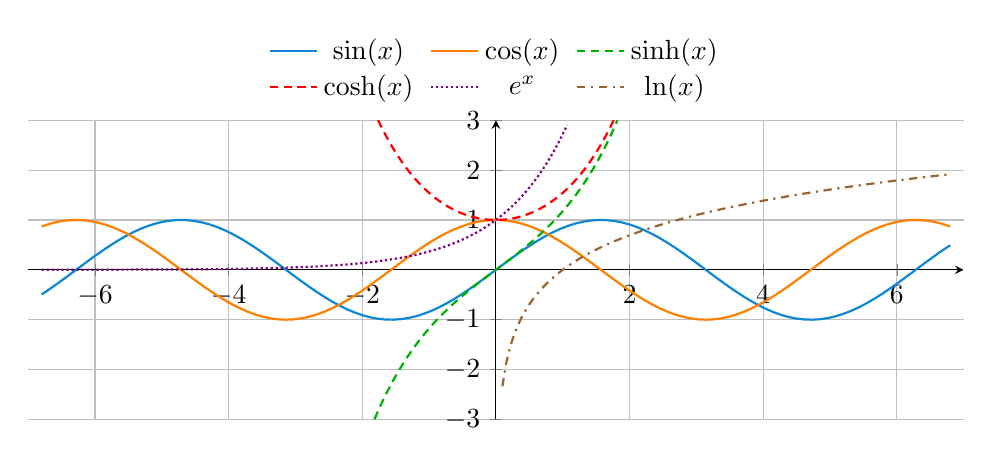
\begin{tikzpicture}[font=\ZSFfontDiagramLabel]
\begin{axis}[
    scale only axis,
    width=\linewidth-7pt,
    height=3.8cm,
    xmin=-7, xmax=7,
    ymin=-3, ymax=3,
    xtick={-6,-4,-2,2,4,6},
    ytick={-3,-2,-1,1,2,3},
    minor tick num=1,
    axis lines=center,
    grid=both,
    legend style={
        at={(0.5,1.03)},
        anchor=south,
        legend columns=3,
        draw=none,
        fill=none,
        font=\ZSFfontDiagramLabelSmall,
        /tikz/every even column/.append style={column sep=0.4em}
    },
    restrict y to domain=-3.05:3.05,
    enlargelimits=false,
    samples=120
]
% sin(x)
\addplot [cyan!70!blue, thick, domain=-6.8:6.8] {sin(deg(x))};
\addlegendentry{$\sin(x)$}
% cos(x)
\addplot [orange, thick, domain=-6.8:6.8] {cos(deg(x))};
\addlegendentry{$\cos(x)$}
% sinh(x)
\addplot [green!70!black, thick, densely dashed, domain=-2.1:2.1] {sinh(x)};
\addlegendentry{$\sinh(x)$}
% cosh(x)
\addplot [red, thick, densely dashed, domain=-2:2] {cosh(x)};
\addlegendentry{$\cosh(x)$}
% e^x
\addplot [violet, thick, densely dotted, domain=-6.8:1.2] {exp(x)};
\addlegendentry{$e^x$}
% ln(x)
\addplot [brown!80!black, thick, dashdotted, domain=0.04:6.8] {ln(x)};
\addlegendentry{$\ln(x)$}

\end{axis}
\end{tikzpicture}
\end{figbox}

\begin{tablebox}[Variablen der Integralnotation]
\begin{ZSFtable}{Z{0.45} Y{1.55}}
    \ZSFheaderRow \ZSFhead{Zeichen} & \ZSFhead{Was bedeutet es?} \\
     $a,b$ & Feste untere und obere Grenze; bei Mehrfachintegralen die äusseren x-Grenzen. \\
    $c,d$ & Feste untere und obere y-Grenze, wenn x- und y-Grenzen unterschieden werden. \\
     $g_{1,2}(x)$ & Unterer und oberer Rand in y-Richtung beim gerade betrachteten x. \\
    $h_{1,2}(x,y)$ & Unterer und oberer Rand in z-Richtung beim gerade betrachteten Punkt $(x,y)$. \\
     $C$ & Weg/Kurve; parametrisiert durch $\vec r(t)$ für $t\in[t_1,t_2]$. \\
    $t$ & Laufvariable entlang einer Kurve; $t_1$ ist der Start und $t_2$ das Ende. \\
     $u,v$ & Zwei frei veränderbare Werte, mit denen Punkte einer Fläche erzeugt werden. \\
    $U$ & Fläche im uv-Koordinatensystem. Jeder Punkt $(u,v)$ auf $U$ wird durch $\tilde r(u,v)$ zu einem Punkt der Fläche $A$ im Raum. \\
     $\vec r(t),\tilde r(u,v)$ & Liefert den Punkt auf $C$ bzw. auf der Fläche $A$ im Raum. \\
    $\vec r_u,\vec r_v$ & Richtungen auf der Fläche: So bewegt sich der Punkt, wenn nur $u$ bzw. nur $v$ verändert wird. \\
     $A$ & Fläche im Raum oder ebenes Flächengebiet; $O_A$ ist ihr Oberflächeninhalt. \\
    $A_1,A_2$ & Einzelne Teile der äusseren Oberfläche eines Körpers $V$. \\
     $V$ & Körper im Raum bzw. sein Volumen; unter dem Dreifachintegral bezeichnet $V$ den Körper. \\
    $\partial A,\partial V$ & Rand der Fläche $A$ bzw. äussere Oberfläche des Körpers $V$. \\
     $\vec n$ & Normalenvektor: zeigt senkrecht von der Fläche weg; bei geschlossenen Körpern nach aussen. \\
    $dA,dO,dV$ & Winziges Flächenstück, Oberflächenstück bzw. Volumenstück, über das aufsummiert wird. \\
     $W,\Phi$ & Ergebnisgrössen: Arbeit bzw. Fluss.
\end{ZSFtable}
\end{tablebox}

% Kapitel-lokale Satzmodi explizit schliessen: \input erzeugt keine Gruppe.
% Ohne diese Rücksetzung liefen Pack-Modus, Anhang-Dichte und gelockerte
% Display-Umbrüche in das Schlusswort weiter.
\allowdisplaybreaks[0]
\ZSFBoxesBreakableOff
\ZSFChapterDensityReset
